\documentclass[slovene,11pt,a4paper]{article}

\usepackage[margin=1.5cm,bottom=3cm,foot=1.5cm]{geometry}
\usepackage{amsmath}
\usepackage{booktabs}
\usepackage{float}
\usepackage{graphicx}
\usepackage{changepage}
\usepackage{subcaption}
\usepackage{multirow}
\usepackage{blindtext}
\usepackage{hyperref}
\usepackage[version=4]{mhchem}
\usepackage[slovene]{babel}


\pagenumbering{gobble}

\begin{document}

\title{3. naloga \\ Določanje elastičnih konstant v nematskem tekočem kristalu}
\author{Tadej Lozej 28242023}
\maketitle

\begin{center}
Praktikum strojnega učenja v fiziki \\
\bigskip
Predavatelj: red. prof. dr. Borut Paul Kerševan \\
Asistent: Jaka Zaplotnik
\end{center}

\newpage

\tableofcontents

\newpage

\pagenumbering{arabic}

\section{Uvod}

Elastične konstante so pomembna lastnost tekočih kristalov. V tej nalogi bomo spoznali potencialen nov način za določitev le-teh v nematskem tekočem kristalu. To bomo storili s pomočjo nevronskih mrež.

V nemarskem tekočem kristalu orientacijski red opišemo z direktorskim poljem $\vec{n}(\vec{r})$. Ta v vsaki točki kaže v smeri lokalne ureditve gradnikov. Direktor je vektor brez glave. To pomeni, da sta smeri $\vec{n}$ ter $-\vec{n}$ ekvivalentni. Harmonično teorijo tekočih nematskih tekočih kristalov začnemo opisovati z Frank-Oseenovo gostoto elastične proste energije.

\begin{equation}
    f_{elastic} =
    \frac{1}{2} K_{11} (\nabla \cdot \vec{n})^2 + 
    \frac{1}{2} K_{22} (\vec{n} \cdot \nabla \times \vec{n})^2 +
    \frac{1}{2} K_{33} (\vec{n} \times \nabla \vec{n})^2,
\end{equation}
kjer so $K_{11}$, $K_{22}$ in $K_{33}$ različne deformacijske konstante. Prvi člen predstavlja pahljačasto deformacijo, drugi zvojno in tretji upogibno.

Eksperimentalno določanje deformacijskih konstant izkorišča odziv tekočega kristala na zunanje električno polje. Konceptualno je preprost ampak eksperimentalno še zdaleč ni trivialen, saj je težko natančno kontrolirati eksperimentalne pogoje in posledično rezultati v literaturi močno variirajo.

Obstaja povezava med elastičnostjo tekočih kristalov ter njihovimi optičnimi lastnostmi. Ureditvena anizortopija povzroči dvolomnost. Svetlobni žarek, ki potuje skozi tekoči kristal lahko razdelimo na redno in izredno komponento. Potovanje rednega žarka ni odvisno od smeri direktorja. Propagacija izrednega žarka pa je odvisna od kota $\theta$ med ravnino, pravokotno na valovni vektor $\vec{k}$, ter direktorjem $\vec{n}$.

Če direktor v smeri osi $z$ spreminja svojo smer je posledično za izredni žarek lomni količnik $n = n(z)$. Posledično dobimo fazni zamik med rednim ter izrednim žarkom, ki je odvisen od profila lomnega količnika. Razlika v fazi je

\begin{eqnarray}
    \Gamma = \frac{2\pi}{\lambda} \int_{0}^{d} (n(z) - n_0)dz,
\end{eqnarray}
kjer je $d$ debelina vzorca, $\lambda$ valovna dolžina svetlobe ter $n_0$ lomni količnik za redni žarek. Če je začetni profil lomnega količnika ustreza neravnovesnemu stanju tekočega kristala se ta relaksira z nekimi karakterističnimi časi, ki so odvisni od elastičnih konstant. Iz časovne evolucije profila lomnega količnika bi lahko na nek način pridobili elastične konstante.

V nalogi obravnavamo enostaven model nematskega tekočega kristala med dvema neskončnima ploščama z dvodimenzionalnim direktorskim poljem

\begin{equation}
    \vec{n}(z) = (\cos \theta (z), 0, \sin \theta (z)).
\end{equation}

Z izbiro sidranja izberemo $\theta (0)$ ter $\theta (d)$. Izraz za gostoto elastične proste energije se poenostavi v

\begin{equation}
    f_{elastic} = 
    \frac{1}{2} K_{11} \left( \frac{\partial n_z}{\partial z} \right)^2 + 
    \frac{1}{2} K_{33} \left( \frac{\partial n_x}{\partial z} \right)^2.
\end{equation}

Zanima nas relaksacija direktorskega polja iz nekega začetnega profila $\theta (z, t=0)$ v ravnovesno stanje $\theta(z, t=\infty)$. To določimo z reševanjem Euler-Lagrangeove enačbe. Dobimo difuzijsko enačbo za relaksacijo $\theta (z, t)$, ki vsebuje obe elastični konstanti.

Funkcije $\theta (z)$ nemoremo eksperimentalno izmeriti. Izmerimo pa lahko intenziteto prepuščene svetlobe skozi vzorec. Pred in za vzorec tekočega kristala postavimo polarizator ($\pi / 4$) ter analizator ($-\pi / 4$). Časovno spreminjanje intenzitete nam da podatek o relaksaciji direktorskega polja, ki je pogojena z elastičnimi konstantami.

Cilj naloge je pokazati, da lahko z dobro naučeno nevronsko mrežo zgolj iz podatka o spreminjanju intenzitete $I(t)$ zanesljivo ter natančno določimo elastične konstante nematskega tekočega kristala.

\section{Podatki}

Na voljo imamo 100000 simulacij. Za vsako simulacijo imamo podan začetni profil orientacije direktirja, vrednost elastične konstante ($K_{11} = K_{22} = K$ v prvem delu naloge sta enaki), intenzitetni profil ter zašumljen intenzitetni profil. Intenzitetni profili so podani za štiri različne vrednosti valovnih dolžin $\lambda = 500, \, 505, \, 700, \, 900 \, \text{nm}$.

Na sliki \ref{fig:Kvalues} lahko vidimo histogram vrednosti elastične konstante $K$ prisotne v simulacijah. Minimalna vrednost je $2 \cdot 10^{-18}$ maksimalna pa $2 \cdot 10^{-11}$. Med tema dvema vrednostima so konstante uporabljene v simulaciji precej enakomerno porazdeljene.

\begin{figure}[h!]
    \centering
    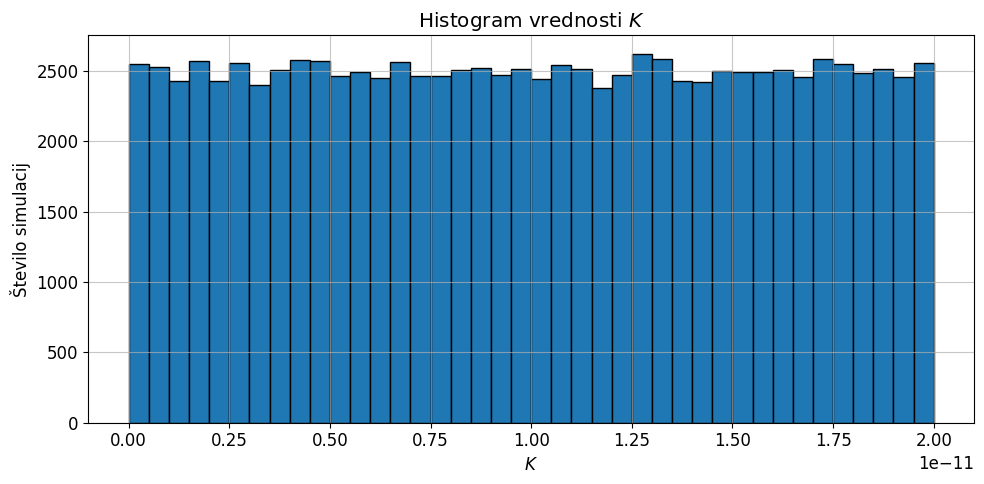
\includegraphics[width=0.9\linewidth]{imgs/Kvalues.png}
    \caption{Porazdelitev vrednosti elastične konstante $K$ uporabljenih v simulacijah.}
    \label{fig:Kvalues}
\end{figure}

\begin{figure}[h!]
    \centering
    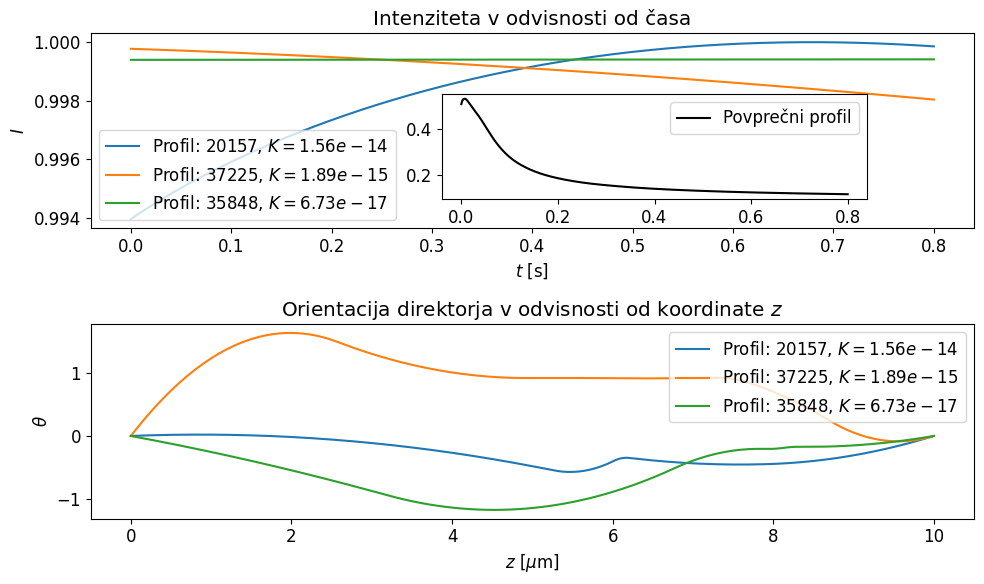
\includegraphics[width=0.9\linewidth]{imgs/odstopanje.png}
    \caption{Profili intenzitete, ki najbolj odstopajo od povprečnega profila.}
    \label{fig:odstopanje}
\end{figure}

Na sliki \ref{fig:odstopanje} lahko zgoraj vidimo tri profile intenzitete, ki najbolj odstopajo od povprečnega profila intenzitete, ki je prikazan v vrinjenem grafu s črno črto. Vsi tri profili so skoraj konstantni. Prav tako imajo vsi tri profili majhne elastične konstante. Te dve lastnosti sta najverjetneje povezani. Majhna elastična konstanta je kriva za počasno relaksacijo. Manjša kot je elastična konstanta počasnejša je relaksacija. Na spodnjem delu slike so prikazani tudi začetni profili orientacije direktorja za vse tri primere.

Našo hipotezo o povezavi velikosti elastične konstante ter času relaksacije lahko vizualno preverimo na sliki \ref{fig:relaksacija}. Na sliki vidimo pet primerov relaksacije začetnega profila na levi ter ustrezne intenzitete v odvisnosti od časa za vse valovne dolžine na desni. Od zgoraj navzdol vrednost elastične konstante narašča. Vidimo, da se na prvi pogled relaksacijski čas krajša. Pri primeru z najmanjšo elastično konstanto se profil praktično sploh ne spremeni. Pri primeru z največjo elastično konstanto se pa profil relaksira zelo hitro.

\begin{figure}[h!]
    \centering
    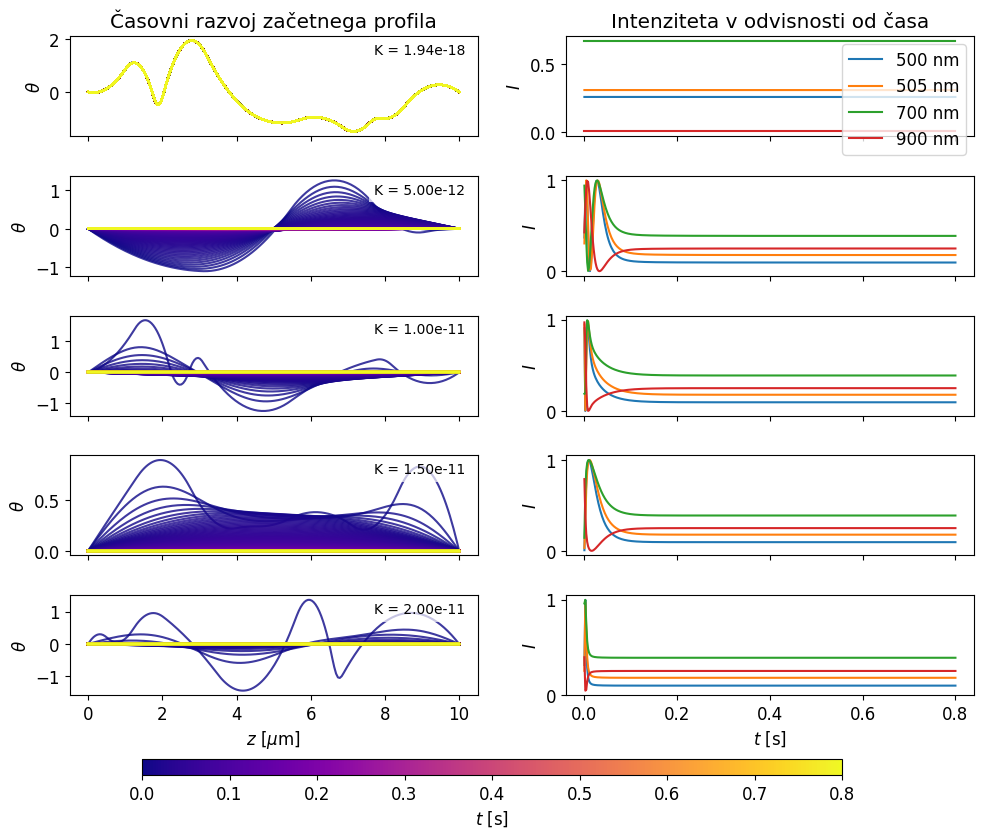
\includegraphics[width=0.9\linewidth]{imgs/relaksacija.png}
    \caption{Profili intenzitete, ki najbolj odstopajo od povprečnega profila.}
    \label{fig:relaksacija}
\end{figure}

\section{Uporaba nevronskih mrež}

Želimo skonstruirati nevronsko mrežo, ki bi za vsak časovni potek intenzitete $I(t)$ znala določiti elastično konstanto $K$. Vhodni podatek mreže je vektor $\vec{X} = [I_{t=0}, I_{t=\Delta t}, ..., I_{t=399\Delta t}]$ izhodni pa $\vec{Y} = [K]$. Eksperimentalno zadostne količine podatkov za učenje nevronske mreže nemoremo doseči, zato se poslužujemo simulacij.

\end{document}